\section{Aplicação Desenvolvida}
Para a primeira entrega do aplicativo, foram desenvolvidos os seguintes requisitos:
\begin{itemize}
    \item Eu, como motorista, gostaria de me cadastrar no sistema para ter acesso ao login
    \item Eu, como motorista, gostaria de logar no sistema para utilizar as funcionalidades do mesmo
    \item Eu, como motorista, gostaria de ver os postos dentro de uma rota para facilitar a minha escolha de posto
\end{itemize}
No Anexo \ref{chap:telas} encontram-se algumas telas da aplicação desenvolvida.

\subsection{Testes Automatizados}

Foram feitos testes de integração e unitários para garantir o funcionamento dos métodos do código-fonte e da integração da aplicação mobile com a API.

Para a aplicação mobile, foram utilizados os \textit{frameworks open source} Jasmine para escrever os testes e o Karma para rodar a suíte. O Karma é um ambiente de teste para Javascript onde os desenvolvedores conseguem \textit{feedbacks} rápidos do código que estão desenvolvendo \cite{karma}. O Jasmine é um \textit{framework} que utiliza conceitos de \textit{behavior-driven development} para escrever testes \cite{jasmine}. O CodeCov foi utilizado para adquirir a cobertura de código dos testes.

Para a API, foi utilizado o RSpec, que é uma ferramenta para escrever e executar a suíte de testes \cite{rspec} e o Coveralls que adquire a cobertura de código dos testes \cite{coveralls}.

\subsection{Métricas de Código-fonte}

Para as métricas de código-fonte da aplicação mobile, foi utilizado o TSLint, que checa código TypeScript em questões de manutenabilidade, leitura e erros funcionais \cite{tslint}.

No código-fonte da API, foi utilizado o CodeClimate, uma ferramenta que baixa o código do Github e checa em seus servidores a complexidade do código, duplicação, estilo e segurança \cite{codeclimate}. O CodeClimate utiliza as seguintes para gerar o relatório final:
\begin{itemize}
    \item \textbf{Reek}, para verificação de \textit{code smells}, que são sintomas no código-fonte que podem gerar problemas;
    \item \textbf{Flog}, para a verificação da complexidade do código Ruby;
    \item \textbf{Rubocop}, que verifica estilo e qualidade do código;
    \item \textbf{Brakeman}, para uma verificação estática de segurança do código;
\end{itemize}

Além disso, é também uma ferramenta própria do CodeClimate para checar duplicações de código.

Adicionalmente, é feita na integração contínua um relatório de métricas pelo Rubocop que impede que a \textit{build} passe caso a complexidade seja maior do que 6, que é o padrão de complexidade ciclomática máxima aceitável. Além de complexidade, o Rubocop possui diversas outras ferramentas embutidas que verificam outros aspectos baseados no guia de estilo do Ruby mantido pela comunidade \cite{rubocop}. Os padrões mínimos ou máximos dessas outras ferramentas serão analisadas com o desenvolvimento do projeto.

No Anexo \ref{chap:metricas} é possível encontrar os resultados da coleta de métricas do sistema.

\subsection{Integração e Deploy contínuo}
Há três tipos de ambientes no desenvolvimento desta aplicação: \textit{development}, \textit{staging} e \textit{production}. O ambiente de \textit{development} ou desenvolvimento, é o ambiente local de cada desenvolvedor, \textit{staging} ou pré produção é um ambiente para serem realizados testes beta e \textit{production} ou produção é o ambiente final onde a aplicação será de fato utilizada pelos usuários.

Na API a integração contínua é feita com a ferramenta TravisCI. Onde, se um \textit{pull request} é aceito na \textit{branch} \textit{staging}, o Travis executa toda a suíte de testes para ver se algum deles pode ter resultado em falha, caso todos passem, ele verifica se todas as métricas definidas pelo Rubocop estão de acordo com o padrão definido. Caso todas as métricas passem, a build de pré produção é criada, o Travis envia as informações de cobertura de testes para o Coveralls, as informações de métricas para o Code Climate e logo em seguida realiza o \textit{deploy} no ambiente de pré produção no Heroku.

Caso um \textit{pull request} seja aceito na \textit{branch} \textit{master} todo o processo será o mesmo, com exceção que o \textit{deploy} irá ocorrer no ambiente de produção no Heroku.

A figura \ref{img:integracao_deploy_continuo_api} ilustra o processo de integração e deploy contínuo feito na API.

\begin{figure}[H]
    \centering
    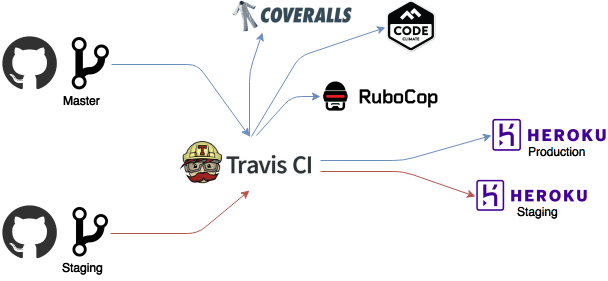
\includegraphics[scale=0.5]{figuras/api_ci.png}
    \caption[Integração e deploy contínuo API]{Integração e deploy contínuo API.}
    \label{img:integracao_deploy_continuo_api}
\end{figure}

No aplicativo, foi planejada a integração e o deploy contínuo para ocorrer da seguinte forma:

\begin{figure}[H]
    \centering
    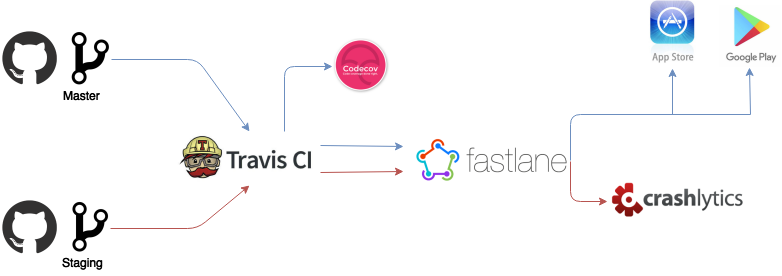
\includegraphics[scale=0.5]{figuras/ci_should_be.png}
    \caption[Integração e deploy contínuo planejado para o APP]{Integração e deploy contínuo planejado para o APP}
    \label{img:integracao_deploy_continuo_planejado_app}
\end{figure}

Se um pull request \textit{pull request} é aceito na \textit{branch} \textit{master}, o Travis irá realizar toda a suíte de testes, caso todos passem enviará as informações de cobertura para o
Codecov e através do Fastlane realizará o deploy do aplicativo tanto na Play Store quanto na App Store. E caso um \textit{pull request} é aceito na \textit{branch} \textit{staging}, todo o processo é repetido, com exceção
que não é realizado o deploy do aplicativo nas lojas e sim no Crashlytics, que irá criar a versão beta do aplicativo e enviará por email para os emails configurados previamente.

Uma vez que o aplicativo ainda não chegou ao estágio de deploy nas lojas, o planejamento para a primeira entrega é só até o deploy beta, como mostrado na figura \ref{img:integracao_deploy_continuo_planejado_primeira_entrega}:

\begin{figure}[H]
    \centering
    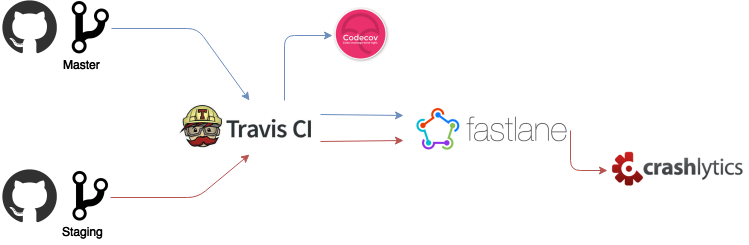
\includegraphics[scale=0.5]{figuras/ci_as_is.png}
    \caption[Integração e deploy contínuo planejado para o APP]{Integração e deploy contínuo planejado para a primeira entrega}
    \label{img:integracao_deploy_continuo_planejado_primeira_entrega}
\end{figure}

Porém não foi possível fazer com que o deploy contínuo aconteça logo após a integração contínua, um desafio causado por escolher desenvolvimento híbridos de aplicativo.
Uma vez que o código versionado do aplicativo é o mesmo código para a plataforma Android e iOS, e após realizar a build desse código é gerado códigos em cada plataforma (não versionados),
a ferramenta de integração contínua não consegue ter acesso aos códigos de cada plataforma para realizar os devidos deploys. Sendo assim, o deploy contínuo está acontecendo manualmente
por enquanto que nenhuma solução ainda foi encontrada, através do comando:

\begin{lstlisting}[language=bash]
  $ fastlane beta
\end{lstlisting}

Sendo assim, a figura \ref{img:integracao_deploy_continuo_atual} ilustra como está funcionando a integração e o deploy contínuo do aplicativo até o presente momento.

\begin{figure}[H]
    \centering
    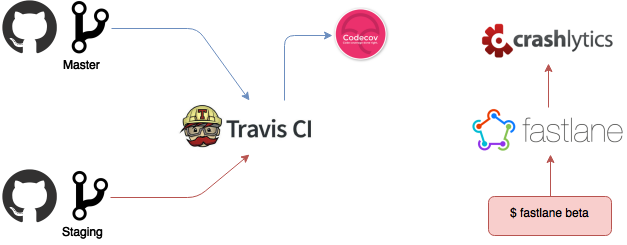
\includegraphics[scale=0.5]{figuras/ci_currently.png}
    \caption[Integração e deploy contínuo atual]{Integração e deploy contínuo atual}
    \label{img:integracao_deploy_continuo_atual}
\end{figure}

